%Fer versio dos pags, i en castellà i amb foto.

\documentclass[a4paper,10pt]{article} % Default font size and paper size


%\usepackage{xunicode,xltxtra,url,parskip} % Formatting packages
\usepackage{url,parskip} % Formatting packages
\usepackage{graphicx}

\usepackage[usenames,dvipsnames]{xcolor} % Required for specifying custom colors

%\usepackage[big]{layaureo} % Margin formatting of the A4 page, an alternative to layaureo can be \usepackage{fullpage}
% To reduce the height of the top margin uncomment: \addtolength{\voffset}{-1.3cm}
\usepackage[left=3.2cm,right=3.2cm,top=2cm,bottom=2.5cm]{geometry}
\usepackage{hyperref} % Required for adding links	and customizing them
\definecolor{linkcolour}{rgb}{0,0.2,0.6} % Link color
\hypersetup{colorlinks,breaklinks,urlcolor=linkcolour,linkcolor=linkcolour} % Set link colors throughout the document
\usepackage{array}
\newcolumntype{R}[1]{>{\raggedleft\let\newline\\\arraybackslash\hspace{0pt}}m{#1}}

\usepackage{titlesec} % Used to customize the \section command
\titleformat{\section}{\scshape\raggedright}{}{0em}{}[\titlerule] % Text formatting of sections
\titlespacing{\section}{0pt}{3pt}{3pt} % Spacing around sections

\begin{document}

\pagestyle{empty} % Removes page numbering

%\font\fb=''[cmr10]'' % Change the font of the \LaTeX command under the skills section

%\vspace{-20pt}

%\begin{center}
%\begin{huge}
%Carlos Segarra
%\end{huge}
%
%\begin{tabular}{c}
%    Polytechnical University of Catalonia  $\cdot$ \href{mailto:carlossegarragonzalez@gmail.com}{carlossegarragonzalez@gmail.com}\\[4pt]
%\end{tabular}
%\end{center}

\section{Personal Information}

\begin{table}[ht]
\begin{minipage}{0.77\linewidth}
    \begin{tabular}{R{2.5cm}p{3cm}}
        Name: & Carlos Segarra \\
        Date of birth: & 09/06/1996 \\
        Place of birth: & Barcelona, Spain \\
        Residence: & Neuchatel, CH \\
        Mail: & carlossegarragonzalez@gmail.com \\
        Phone: & +41 79 935 95 41
    \end{tabular}
\end{minipage}\hfill
\begin{minipage}{0.2\linewidth}
\centering
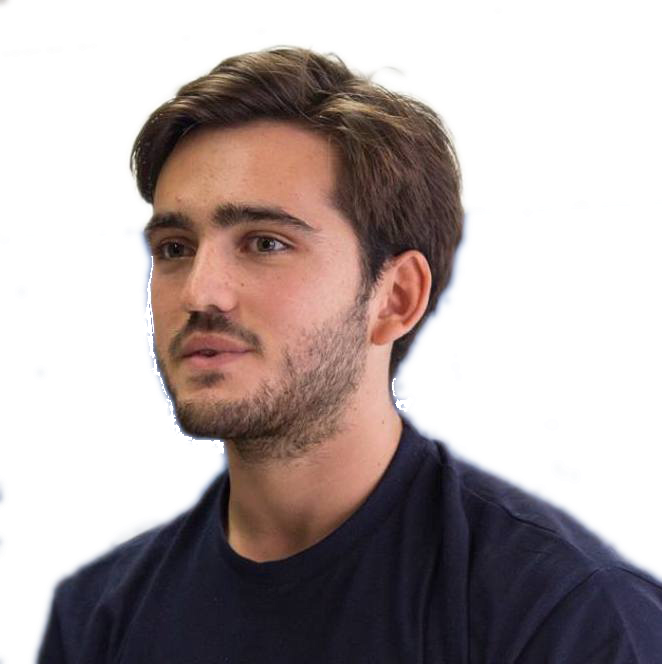
\includegraphics[width=2.5cm]{carlos_portrait.png}
\end{minipage} 
\end{table}

\section{Work Experience}
%
\begin{tabular}{R{2.5cm}|p{11.5cm}}
    \emph{Current} & Trainee at \textsc{CSEM} \\
    \textsc{June 2018} & \small{\emph{Embedded Software Division} - Sup. Ricard Delgado Gonzalo, PhD }\\ 
& \footnotesize{Summer internship at the the Cybersecurity department at Nokia Bell Labs in Paris-Saclay, France. There, I worked in Bitcoin's Blockchain security. We defined, designed and implemented a modelling scheme for malicious transaction and their derived chains. With this abstraction model we identified servicies within the Bitcoin ecosystem and we applied it to identity-oriented address clustering. }
\end{tabular}

\begin{tabular}{R{3cm}|p{11cm}}
    \textsc{September 2018} & Trainee at \textsc{Nokia Bell Labs} \\
    \textsc{June 2018} & \small{\emph{Security Group} - Sup. Matteo Signorini, PhD and Matteo Pontecorvi, PhD}\\ 
& \footnotesize{Summer internship at the the Cybersecurity department at Nokia Bell Labs in Paris-Saclay, France. There, I worked in Bitcoin's Blockchain security. We defined, designed and implemented a modelling scheme for malicious transaction and their derived chains. With this abstraction model we identified servicies within the Bitcoin ecosystem and we applied it to identity-oriented address clustering. }
\end{tabular}

\begin{tabular}{R{2.5cm}|p{11.5cm}}
\textsc{June 2018} & Research Student at \textsc{Barcelona Supercomputing Center} \\
    \textsc{Apr 2017} & \small{\emph{Workflows and Distributed Computing Group} - Sup. Rosa M. Badia, PhD} \\ 
& \footnotesize{The workflows and distributed computing group at the Barcelona Supercomputint Center located in Barcelona, Spain, develops a programming framework, \href{https://www.bsc.es/research-and-development/software-and-apps/software-list/comp-superscalar/}{COMPSs}, which aims to ease the development of applications for distributed architectures. During my work there, I developed clustering algorithms in the Python binding of the software to test the scalability of the framework as well as new functionalities. All the executions were performed in the Mare Nostrum 4 supercomputer, enabling the use of bigger datasets and greater computational resources.}
\end{tabular}

\section{Education}

\begin{tabular}{rl}	
\textsc{July} 2018 & Bachelor's degree in \textsc{Mathematics} \\ & \textbf{Polytechnic University of Catalonia}, UPC\\

%------------------------------------------------

\textsc{July} 2018 &  Bachelor`s degree in \textsc{Telecomunications Science and Technology}\\ & \textbf{Polytechnic University of Catalonia}, UPC\\

\textsc{July} 2018 &  Degree in \textsc{Multidisciplinar Engineering} \textbf{CFIS}, UPC\\

%------------------------------------------------

\textsc{May} 2014 & Spanish Baccalaureate at \textbf{Escola Betània-Patmos}, Barcelona \\ &  Graduated with honors. \\
\end{tabular}


%----------------------------------------------------------------------------------------
%	EXTRACURRICULAR COURSEWORK
%----------------------------------------------------------------------------------------

\section{Extracurricular Coursework}
\begin{tabular}{rl}	
\textsc{September} 2017 &  Course in \textsc{Bitcoin and Cryptocurrency Technologies} \\
 & \textbf{Princeton}, Coursera\\

\textsc{March} 2017 &  Course in \textsc{Machine and Deep Learning} \textbf{CFIS}, UPC\\

\textsc{January} 2017 &  Course in \textsc{Machine Learning} \textbf{Stanford}, Coursera\\

%------------------------------------------------

\textsc{Summer} 2015 & Abroad summer student at the \textbf{University of Leeds}, U.K\\
& Module in \textsc{Smartphone Applications}\\ & Module in \textsc{Introduction to robotics and Autonomous Systems}\\
\end{tabular}
%----------------------------------------------------------------------------------------
%	SCHOLARSHIPS AND ADDITIONAL INFO
%----------------------------------------------------------------------------------------
\vspace{-5pt}

\section{Scholarships and Certificates}

\begin{tabular}{rl}
\textsc{May} 2015 & Partial tuition fee for the Sudy Abroad \footnotesize (CFIS) \normalsize \\
\textsc{January} 2015 & Economical reward for University Acces Exams \\
 &  (Fundació Catalunya Caixa - La Pedrera) \\
\textsc{June} 2014 & BSc in Mathematics full tuition scolarship
	\footnotesize (CFIS) \normalsize \\
\textsc{May} 2014 & First University Year Scholarship \footnotesize(Generlitat de Catalunya)\normalsize\\
\textsc{March} 2014 & Certificate in Advanced English \footnotesize (Grade A, 84/100) \normalsize \\
\textsc{June} 2012 & Zertifikat A2 (German language) \footnotesize (Grade: 75/80) \normalsize \\
\end{tabular}

%----------------------------------------------------------------------------------------
%	LANGUAGES
%----------------------------------------------------------------------------------------

\section{Languages}

\begin{tabular}{rl}
\textsc{English:} & Very fluent. Level C2.\\

\textsc{German:} & Fluent. Currently at level B2.\\

\textsc{Spanish and Catalan:} & Native competence.\\
\end{tabular}

%----------------------------------------------------------------------------------------
%	COMPUTER SKILLS 
%----------------------------------------------------------------------------------------

\section{Skills and Interests}

\begin{tabular}{rl}
Programming:  & Algorithm-wise \textsc{C++}, Multi-Thread \textsc{Java}, Data Science and ML \textsc{Python}. \\
 &  Numerical Mathematics with \textsc{Matlab}, \textsc{R} and \textsc{Ampl} \\
 Research Interests: & Big Data, cryptography and cryptocurrencies and IT security. \\
Personal Interests: & Sport, Literature, Programming and Travelling.
\end{tabular}

%\section{Skills and Relevant Coursework}
%\begin{tabular}{rl}
%\textsc{Mathematics:} & Discrete Mathematics, Probability, Algebra \\
%\textsc{Computer Science:} & Algorithmics, Object Oriented Programming,  Network Application And Services \\ &
% Introduction to Communications, Machine Learning \\
%\end{tabular}

\section{Awards and Merits}
\begin{tabular}{rl}
\textsc{November} 2016 & 2017 IEEE AP-S Design Contest Applicant \\
 & Desiged an antenna for a CubeSat. \\
\textsc{October} 2016 & Designed an Award-Winning Hack at HackUPC Fall 2016
\end{tabular}

%----------------------------------------------------------------------------------------
%	INTERESTS AND ACTIVITIES
%----------------------------------------------------------------------------------------
%Nomes per CV més informals
%\section{Interests and Activities}
%
%\begin{tabular}{rl}
%Sport: & really sportive person. Practice all kinds of sports almost on a daily basis. \\
%Literature: & interested in the theory of thought politics and philosophy in general. \\
%Teaching: & I consider teaching one of the best ways of learning and so I spend some of \\ & my free time helping younger students. \\
%Logical problems: & apart from my studies I also enjoy solving mathematical and logical puzzles \\ & aswell as programming in my spare time. \\
%
%	
%\end{tabular}

%----------------------------------------------------------------------------------------

\newpage

%----------------------------------------------------------------------------------------
%	GRADE TABLES
%----------------------------------------------------------------------------------------

%\par{\centering\Large \hypertarget{grds}{Master of Science in \textsc{Finance}}\par}\large{\centering Grades\par}\normalsize
%
%\begin{center}
%\begin{tabular}{lcc}
%\multicolumn{1}{c}{\textsc{Exam}} & \textsc{Grade}&\textsc{Credit Hrs}\\ \hline
%Corporate Finance (Valuation) & 25 & 6\\
%Financial Statement Analysis & 28 & 6\\
%Statistics & 27 & 6\\
%Theory of Finance & 26 & 6\\
%Quantitative Methods for Finance & 30 & 6\\
%Econometrics & 24 & 6\\
%Derivatives & 31 & 6\\
%Management of Financial and Insurance Companies & 30 & 6\\
%Business Law & 31 & 6\\
%Investment Banking	& 28 & 6\\ \\		
%Behavioral Models for Economics and Finance	 & 29 & 6\\
%Numerical Methods for Finance & 29 & 6\\
%Advanced Derivatives & 30 & 6\\
%Fixed Income (Advanced Methods) & 30 & 6\\ \\
%English Language & 30 &	4\\
%French Language & 31 &	4\\	
%Internship & & 8\\		
%Final Thesis & & 20\\	
%& Total & 120\\\cline{2-3}
%&\textsc{Gpa}&\textbf{8.0}
%\end{tabular}
%\end{center}
%\bigskip
%\hrule
%\bigskip
%
%%------------------------------------------------
%
%\bigskip
%
%\par{\centering\Large \hypertarget{grds_usc}{Exchange Program at \textsc{usc}, Los Angeles}\par}\large{\centering Grades\par}\normalsize
%
%\begin{center}
%\begin{tabular}{lcc}
%\multicolumn{1}{c}{\textsc{Exam}} & \textsc{Grade} & \textsc{Grade Points}\\ 
%\hline
%Corporate Financial Strategy & A & 4\\
%Derivatives & A & 4\\
%Money, Credit, and Banking & A & 4\\
%Business Strategy & A- & 3.5\\
%& &\\\cline{2-3}
%& \textsc{Gpa} & \textbf{3.875}
%\end{tabular}
%\end{center}

%----------------------------------------------------------------------------------------

\end{document}
